% -*- TeX-master: "oving04"; -*-
\oppgaver{6}

\begin{oppgave}
Regn ut determinanten til følgende matriser og avgjør -- basert på
dette -- om kolonnene er lineært uavhengige:
\begin{punkt}
$
\begin{bmatrix}
1 & 2\\
1 & 2
\end{bmatrix}
$
\end{punkt}
\begin{punkt}
$
\begin{bmatrix}
1 & 2\\
2 & 1
\end{bmatrix}
$
\end{punkt}
\begin{punkt}
$
\begin{bmatrix}
2 & -5 & 3 & 4 & 0 \\
2 & -4 & 7 & 2 & 1 \\
-6 & 15 & -9 & -12 & 1 \\
4 & -8 & 14 & 5 & -6 \\
-2 & 5 & 4 & 5 & -4
\end{bmatrix}
$
\end{punkt}
\end{oppgave}

\begin{losning}
\begin{punkt}
Determinanten er~$0$, kolonnene er lineært avhengige.
\end{punkt}

\begin{punkt}
Determinanten er~$-3$, kolonnene er lineært uavhengige.
\end{punkt}

\begin{punkt}
Determinanten er~$-14$, kolonnene er lineært uavhengige.
(Her kan det være lurt å bruke radoperasjoner for å beregne determinanten.)
\end{punkt}

\end{losning}


\begin{oppgave}
Skisser parallellogrammet utspent av følgende vektorer i $\R^2$, og
regn ut arealet.
\begin{punkt}
$\vv{1}{2}$, $\vv{2}{1}$
\end{punkt}
\begin{punkt}
$\vv{1}{1}$,
$\vv{2}{2}$
\end{punkt}
\end{oppgave}

\begin{losning}

\begin{punkt}
3

\begin{center}
	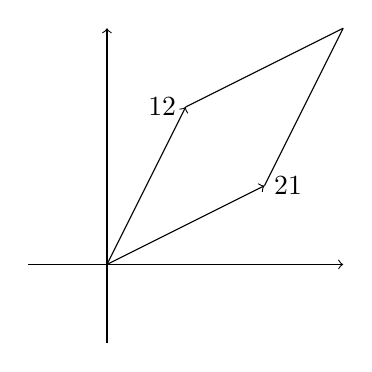
\begin{tikzpicture}[scale=1]
	\draw[->,left] (0,0) node{} -- (1,2) node{$\vv{1}{2}$};
	\draw[->, right] (0,0) node{} -- (2,1) node{$\vv{2}{1}$};
	\draw[] (1,2) node{} -- (3,3);
	\draw[] (2,1) node{} -- (3,3);
	%\draw[->, right] (0,0) node{} -- (2,-1) node{$\V{v}_3$};
	\draw[->] (-1,0) {} -- (3,0) {};
	\draw[->] (0,-1) {} -- (0,3) {};
	\end{tikzpicture}
\end{center}
\end{punkt}

\begin{punkt}
0


\begin{center}
	\begin{tikzpicture}[scale=1]
	\draw[->,above] (0,0) node{} -- (1,1) node{$\vv{1}{1}$};
	\draw[->, right] (0,0) node{} -- (2,2) node{$\vv{2}{2}$};
	%\draw[->, right] (0,0) node{} -- (2,-1) node{$\V{v}_3$};
	\draw[->] (-1,0) {} -- (3,0) {};
	\draw[->] (0,-1) {} -- (0,3) {};
	\end{tikzpicture}
\end{center}
\end{punkt}

\end{losning}


\begin{oppgave}
Regn ut volumet av tetraederet i $\R^3$ med
\[
(8,8,4),\quad
(16,0,0),\quad
(1,1,9)
\quad\text{og}\quad
(8,11,-4)
\]
som hjørner.
\end{oppgave}

\begin{losning}
430

\noindent
Hint: Velg et referansepunkt og se på differansen fra de andre vektorene. Du har nå tre vektorer i $\mathbb{R}^3$ som definerer $T$. Observer at $T$ er en sjettedel av volumet til parallellepipedet definert av vektorene. 
\end{losning}


\begin{oppgave}
La $\V{e}_1$ og~$\V{e}_2$ være enhetsvektorene i~$\R^2$:
\[
\V{e}_1 = \vv{1}{0}
\qquad\text{og}\qquad
\V{e}_2 = \vv{0}{1}
\]
% La $\V{e}_1 = \bigl[ \begin{smallmatrix} 1 \\ 0 \end{smallmatrix} \bigr]$
% og~$\V{e}_2 = \bigl[ \begin{smallmatrix} 0 \\ 1 \end{smallmatrix} \bigr]$
% være enhetsvektorene i~$\R^2$.
En $2 \times 2$-matrise $A$ kan beskrives ved hjelp av fire tall
$\alpha_1$, $\alpha_2$, $\theta$ og~$\varphi$, der:
\begin{align*}
\alpha_1\ &\text{er lengden av vektoren $A \V{e}_1$} \\
\alpha_2\ &\text{er lengden av vektoren $A \V{e}_2$} \\
\theta  \ &\text{er vinkelen (mot klokken) opp til vektoren $A \V{e}_1$} \\
\varphi \ &\text{er vinkelen (mot klokken) fra $A \V{e}_1$ til $A \V{e}_2$}
\end{align*}
Disse er illustrert på figuren under.
\begin{center}
\begin{tikzpicture}[scale=.75]
\draw[->] (-1,0) -- (10,0);
\draw[->] (0,-.2) -- (0,4.5);
\draw[->] (0,0) -- (6,3.46);
\draw[->] (0,0) -- (1.73,3);
\node[anchor=west] at (6,3.46) {$A \V{e}_1$};
\node[anchor=south] at (1.73,3) {$A \V{e}_2$};
\centerarc[](0,0)(0:30:2);
\centerarc[](0,0)(30:60:2.3);
\node at (2.4,0.7) {$\theta$};
\node at (2,1.9) {$\varphi$};
\node at (4.5,2) {$\alpha_1$};
\node at (0.5,2) {$\alpha_2$};
\end{tikzpicture}
\end{center}
\begin{punkt}
Hvordan kan du, basert på tallene $\alpha_1$, $\alpha_2$, $\theta$
og~$\varphi$, se om determinanten til~$A$ er positiv, negativ
eller~$0$?
\end{punkt}
\begin{punkt}
Forklar hvordan determinanten til~$A$ endrer seg hvis vi endrer én av
de fire verdiene $\alpha_1$, $\alpha_2$, $\theta$ og~$\varphi$, mens
vi lar de tre andre forbli som de er.
\end{punkt}
\begin{punkt}
Finn $\det A$ uttrykt ved $\alpha_1$, $\alpha_2$, $\theta$
og~$\varphi$.
\end{punkt}
\end{oppgave}

\begin{losning}
Vi kan anta at vinklene $\theta$ og~$\varphi$ ligger i intervallet
$[-\pi,\pi)$.
\begin{punkt}
Det er kun vinkelen $\varphi$ som har noe å si for om determinanten er
positiv, negativ eller~$0$.  Determinanten er~$0$ hvis $\varphi$
er~$0$ eller~$-\pi$, og ellers har determinanten samme fortegn
som~$\varphi$.
\end{punkt}
\begin{punkt}
Hvis vi øker $\alpha_1$ eller $\alpha_2$, så øker determinanten; hvis
vi minsker en av disse, så minker determinanten.

Hvis vi varierer $\varphi$ innenfor intervallet $[-\pi/2, \pi/2]$, så
øker determinanten når $\varphi$ øker.  I intervallene $[-\pi,-\pi/2]$
og $[\pi/2,\pi)$ er det omvendt.

Å variere $\theta$ har ingen effekt på determinanten.
\end{punkt}
\begin{punkt}
$\det A = \alpha_1 \alpha_2 \sin \varphi$
\end{punkt}
\end{losning}



\begin{oppgave}
La $A$ være matrisen \[
\begin{bmatrix}
\;a & b & 0 & 0\;\\
\;c & 0 & 0 & 0\;\\
\;0 & 0 & 0 & x\;\\
\;0 & 0 & y & z\;
\end{bmatrix}.
\]
\begin{punkt}
Finn $\det A$ uttrykt ved $a, b, c$ og $x, y, z$.
\end{punkt}

\begin{punkt}
For hvilke $a, b, c$ og $x, y, z$ er $A$ inverterbar?
\end{punkt}
\end{oppgave}


\begin{losning}

\begin{punkt}
$bcxy$
\end{punkt}

\begin{punkt}
Vi må ha at $b$, $c$, $x$ og~$y$ alle ikke er lik null.
\end{punkt}

\end{losning}

\begin{oppgave}
Avgjør om følgende påstander er sanne eller ikke. Gi et bevis eller moteksempel i hvert tilfelle.

\begin{punkt}
La $A$ og $B$ være $n\times n$-matriser. Hvis $AB$ er inverterbar, så er både $A$ og $B$ inverterbare.
\end{punkt}

\begin{punkt}
Anta at $A$ er en inverterbar matrise. Da har vi at $$\text{det}(A^{-1})=\frac{1}{\text{det}(A)}.$$
\end{punkt}

\begin{punkt}
Hvis $A$ og~$B$ er $n \times n$-matriser, så er
\[
\det (A + B) = \det A + \det B.
\]
\end{punkt}

\begin{punkt}
Hvis $A$ og~$B$ er $n \times n$-matriser, så er
\[
\det (AB) = \det (BA).
\]
\end{punkt}

\end{oppgave}

\begin{losning}

\begin{punkt}
Sant.

\noindent
Hint: En matrise er inverterbar hvis og bare hvis determinanten ikke er lik null. Vi vet også at $\text{det}(AB)=\text{det}(A)\text{det}(B)$. Vi har antatt at $\text{det}(AB)\neq 0$. Kan du fullføre beviset?
\end{punkt}

\begin{punkt}
Sant.

\noindent
Hint: $AA^{-1}=I$ og $\text{det}(AB)=\text{det}(A)\text{det}(B)$.
\end{punkt}

\begin{punkt}
Usant.
\end{punkt}

\begin{punkt}
Sant.  Produktregelen for determinant gir:
\[
\det (AB)
 = (\det A)(\det B)
 = (\det B)(\det A)
 = \det (BA)
\]
\end{punkt}

\end{losning}


\begin{oppgave}
La $A$ være en $n \times n$-matrise, og la $\V{u}$ og~$\V{v}$ være
vektorer i~$\R^n$.  Anta at $\V{u} \ne \V{v}$, men at
$A \V{u} = A \V{v}$.  Hva kan du da si om determinanten til~$A$?
\end{oppgave}

\begin{losning}
Determinanten må være lik null.

\noindent
Hint: Vi antar at $A\V{u}-A\V{v}=0$ for $\V{u}-\V{v}\neq 0$. Ved regnereglene for matriser blir dette $A(\V{u}-\V{v})=0$. Likningen $A\V{x}=\V{0}$ har altså en ikke-triviell løsning; $\V{x}=\V{u}-\V{v}$. Dette betyr -- fra Teorem \ref{thm:linuavh} -- at kolonnene til $A$ er lineært avhengige. Hva kan du nå si om determinanten til $A$?
\end{losning}


\begin{oppgave}
La $A$ være en $m \times n$-matrise slik at
\[
\det (A\tr \cdot A) \ne 0.
\]
Hva kan du da si om $m$ og~$n$?
\end{oppgave}

\begin{losning}
$m\geq n$.

\noindent
Skisse til løsning: Hva skjer hvis vi antar $m<n$? Svar: Siden kolonnene til $A$ er vektorer i $\mathbb{R}^n$ og vi har $n>m$ vektorer, må kolonnene til $A$ være lineært avhengige. Husk at $$A\tr A=\begin{bmatrix}
\V{a}_1\tr \V{a}_1 & \V{a}_1\tr \V{a}_2 & \cdots & \V{a}_1\tr\V{a}_n\\
\V{a}_2\tr \V{a}_1 & \V{a}_2\tr \V{a}_2 & \cdots & \V{a}_2\tr\V{a}_n\\
\vdots & \vdots & \ddots & \vdots\\
\V{a}_n\tr \V{a}_1 & \V{a}_n\tr \V{a}_2 & \cdots & \V{a}_n\tr\V{a}_n
\end{bmatrix},
$$ hvor $\V{a}_1,\dots,\V{a}_n$ er kolonnene til $A$. Du kan nå bruke at kolonnene til $A$ er lineæret avhengige til å argumentere for at kolonnene til $A\tr A $ er lineært avhengige. Derfor må determinanten være lik null.
\end{losning}


\begin{oppgave}
La $A$ være følgende matrise:
\[
A =
\begin{bmatrix}
 3 & 0 & 2 & -2 & 1 & 0 & 1 & -1 \\
-1 & 1 & 5 &  1 & 4 & 1 & 1 &  2
\end{bmatrix}
\]
Finn $\det (A \cdot A\tr)$ og $\det (A\tr \cdot A)$.
\end{oppgave}

\begin{losning}
$\det (A \cdot A\tr)=936$, $\det (A\tr \cdot A)=0$.
\end{losning}
